\section{BEHAVIORAL PATTERNS}
\subsection{Strategy}
Strategy pettern permit the definitions of many algorithms which served the same purpose. In this case, we used strategy patterns to define the way of calculating the price of the reservations. As mentioned in the previous section, we have implemented four decorators, two for flight reservation, two for hotel reservation. There're also four strategy classes corresponding to the decorators.

\begin{figure}[h]
\centering
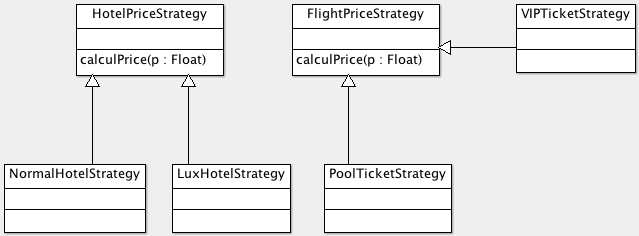
\includegraphics[width=12cm]{project/images/strategy.png}
\caption{Class diagram of strategies}
\end{figure}

\paragraph{}
Take an example of flight reservation's price's calculation. The method \textit{calculPrice} from two strategies are
\begin{lstlisting}
public class CheapHotelStrategy implements HotelPriceStrategy {
...
	@Override
	public float calculPrice(float p) {
		// TODO Auto-generated method stub
		return p * 80f / 100f;
	}
...
}

public class LuxHotelStrategy implements HotelPriceStrategy {
...
	@Override
	public float calculPrice(float p) {
		// TODO Auto-generated method stub
		return p * 120f / 100f;
	}
...
}
\end{lstlisting}

\subsection{Observer}


\subsection{Iterator}

\subsection{Visitor}

\subsection{Template}